\documentclass{article}
\usepackage{amsmath,amssymb,amsfonts}
\usepackage{latexsym}
\usepackage{graphicx}
\usepackage{verbatim}
\usepackage{booktabs}
\usepackage[usenames,dvipsnames,svgnames,table]{xcolor}
\usepackage{todonotes} % Required for the boxes that questions appear in

\newcommand{\mybox}[1]
{
\par\noindent
\todo[inline, backgroundcolor=SkyBlue!40,bordercolor=SkyBlue,size=\large]{\textbf{#1}}
\vspace{1em}
}

\usepackage[top=25mm, bottom=25.4mm, left=16.7mm, right=18.9mm]{geometry}

\usepackage{fancyhdr}
\pagestyle{fancy}
\lhead{Numerical Analysis Assignment \#3 }
\chead{Xinglu Wang \quad 3140102282}
%\renewcommand{\headrulewidth}{0.3pt}

\usepackage[framed,numbered,autolinebreaks,useliterate,final]{mcode}
\usepackage{listings}
\title{\textbf{Numerical Analysis Assignment \#3}}
\author{Xinglu Wang \qquad Student Number: 3140102282
    \\ %\vspace{0.5em}
    College of Information Science \& Electronic Engineering}
\date{}

\makeatletter
\def\@seccntformat#1{%
  \expandafter\ifx\csname c@#1\endcsname\c@section\else
  \csname the#1\endcsname\quad
  \fi}
\makeatother

\usepackage{multirow}

\usepackage{sectsty}
\sectionfont{\color{NavyBlue}\selectfont}
\subsectionfont{\color{SkyBlue}\itshape\selectfont}

\newcommand{\abs}[1]{\left| #1 \right| }
\newcommand{\norm}[1]{\left\| {#1} \right\|}

\begin{document}
\maketitle
\section{Problem 1}
The following linear system $A\bf{x}=\bf{b}$ have $\bf{\tilde x}$ as the actual solution and $\bf{x}$ as an approximate solution. Compute $\norm{\bf{x}-\bf{\tilde x}}_\infty $ and $\norm{A\bf{\tilde x}-\bf{b}}_\infty$.
\begin{description}
  \item[a). Solution:]
According to the definition of norm:
\begin{eqnarray*}
    {\bf{x}}&=&(0,-7,5)^t, \\
  {\bf{\tilde x}}&=&(-0.2,-7.5,5.4)^t
\end{eqnarray*}
\begin{equation}
\Rightarrow
\norm{\bf{x}-\bf{\tilde x}}_\infty = \norm{(0.2,0.5,-0.4)}_\infty=max(0.2,0.5,-0.4)=0.5
\end{equation}
First, applied equation with specific number,
\begin{eqnarray*}
  x_1+2x_2+3x_3 &=& 1 \\
  2x_1+3x_2+4x_3 &=& -1 \\
  3x_1+4x_2+6x_3 &=& 2\\
\end{eqnarray*}
We get
\begin{equation*}
A{\bf{\tilde x}}-b=
\left[ {
\begin{array}{c}
0\\
-0.3\\
-0.2
\end{array}
} \right]
\end{equation*}
Then, the norm of residual vector for $\bf{\tilde x}$ is
\begin{equation}
\norm{A\bf{\tilde x}-\bf{b}}_\infty = 0.3
\end{equation}
\item[b). Solution:]
Similarly,
\begin{equation}
  \norm{\bf{x}-\bf{\tilde x}}_\infty = \norm{(0.33,0.9,-0.8)}_\infty=max(0.33,0.9,-0.8)=0.9
\end{equation}
and the norm of residual vector for $\bf{\tilde x}$ is
\begin{equation}
\norm{A\bf{\tilde x}-\bf{b}}_\infty  = \norm{(0.27,0.16,0.21)}_\infty=0.27
\end{equation}

\end{description}
\section{Problem 2}
Show that if $A$ is symmetric, then $\norm{A}_2=\rho (A)$
\\ \textbf{Prove:}
First, we know, if $A$ is a $n\times n$ matrix, then
\begin{equation}
\norm{A}_2 = \left[ \rho(A^T A) \right]^ {\frac{1}{2}}
\end{equation}
 where $\rho $ is the spectral radius defined by $\rho (A) = max \abs{\lambda} $.
 \\Therefore, we just need to prove $\rho(A^T A)=\rho(A)^2$
 \\Assume $\lambda$ is the eigenvalue of $A^T$, then \[
 (AA^T-\lambda^2 I)x=(A^TAx-A^2x)=0 \text{ \quad ,where } A=A^T
 \]
 thus
 \begin{equation}
 \rho(A^T A)= max(\lambda^2) = \rho(A)^2
 \end{equation}
 \[\Rightarrow \norm{A}_2 = \left[ \rho(A^T A) \right]^ {\frac{1}{2}}=\rho (A) \]
\section{Problem 3}
Implement the algorithm of Gaussian elimination with scaled partial pivoting, and solve the following linear systems.
\begin{center} 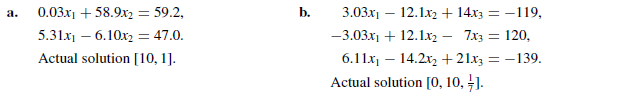
\includegraphics[width=13.5cm]{../pic/p3.png} \end{center}
\textbf{Solution:}
My solution is shown below, and we can find that there still some round\-off error, although applying scaled partial strategies:
My implement of  algorithm of Gaussian elimination is shown below. In the process of make lots of mistakes, and find many skills in matlab, for example \mcode{[~,p]} to discard an output argument.
\begin{center}\begin{tabular}{cccc}
\toprule
\multicolumn{2}{c}{problem a}&\multicolumn{2}{c}{problem b}\\
\midrule
my answer&actual solution&my answer &actual solution \\
\midrule
10.000000000000142&10&-0.000000000000004&0\\
\midrule
1.000000000000000&1& 9.999999999999998&10\\
\midrule
&&  0.142857142857141&1/7\\
\bottomrule
\end{tabular}
\end{center}
\begin{lstlisting}
format long;
clear
A=[0.03 58.9 ;...
	5.31 -6.10];
b=[59.2;...
	47];
res3_1=GauEli([A,b])
A=[3.03 -12.1 14 -119;-3.03 12.1 -7 120; 6.11 -14.2 21 -139];
res3_2=GauEli(A)
%tt=linsolve(A(:,1:end-1),A(:,end))
\end{lstlisting}
\lstinputlisting{../mcode/GauEli.m}
\section{Problem 4}
Implement the Jacobi iterative method and list the first three iteration results when solving the following linear systems, using x(0) = 0.
\begin{center} 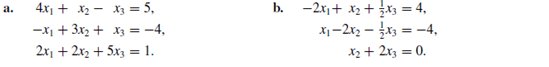
\includegraphics[width=13.5cm]{../pic/p4.png} \end{center}
As what is shown below, I make an comparison with the fractional solution, and find the TOL is satisfied, which means iterative method is just an method to approach true value, but can never be accurate. But it is easier and more relaxing to implement compared with Guass method.
\begin{center}
    \begin{tabular}{lll}\toprule
                    My answer with $TOL=10^-5$  & Accurate answer & Numerical true value \\ \midrule
                   $1.447762108787455$ &  $97/67$ &  1.4477611940298507462686567164179 \\
                   $-0.835818363310185$ & $ -56/67$ & -0.83582089552238805970149253731343 \\
                   $-0.044779294108796$ & $-3/67$ & -0.044776119402985074626865671641791 \\ \bottomrule
     \end{tabular}
  \end{center}
Thus, for problem a). my answer is \begin{equation}
\left[ {\begin{array}{*{20}{c}}
{ - 1.454543254562683}\\
{{\rm{\;}}1.454543254562683}\\
{ - 0.727274337771892}
\end{array}} \right]
\end{equation}
And for problem b). my answer is
\begin{equation}{\rm{ }}\left[ \begin{array}{l}
{\rm{1}}{\rm{.454543254562683}}\\
{\rm{ - 1}}{\rm{.454543254562683}}\\
{\rm{ - 0}}{\rm{.727274337771892}}
\end{array} \right]\end{equation}
\begin{lstlisting}
%% %% problem 4
clear;
A1 = [4,1,-1;-1,3,1;2,2,5];
b1 = [5;-4;1];
res=JacSol(A1, b1)

%y=sym('y',[3,1]);
%[y1,y2,y3]=solve(A1*y==b1) %symbolic computation. Get fractional solution
%vpa([y1;y2;y3])

A2 = [-2,1,0.5;1,-2,-0.5;0,1,2];
b2 = [4;-4;0];
res=JacSol(A2, b2)
\end{lstlisting}

\lstinputlisting{../mcode/JacSol.m}
\section{Problem 5}
Use the Jacobi method and Gauss-Seidel method to solve the following linear systems, with TOL = 0.001 in the L $\infty$ norm.

 \begin{center} 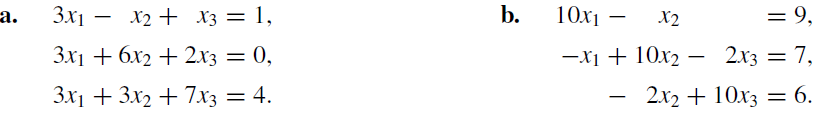
\includegraphics[width=11.5cm]{../pic/p5.png} \end{center}
First, my answer for applying different method and its difference is shown below.
\begin{description}
  \item[a).]

\begin{center}
    \begin{tabular}{lll}\toprule
                    result using JacSol  & result using GauSei & difference between two results \\ \midrule
                      0.035087676431390 & 0.035088637820252 & 0.000000961388862\\
                        -0.236842566509242 &-0.236841914529931 & 0.000000651979311\\
                        0.657894221182574 & 0.657894261447005 & 0.000000040264431\\ \bottomrule
     \end{tabular}
\end{center}
  \item[b).] 
  \begin{center}
    \begin{tabular}{lll}\toprule
                    result using JacSol  & result using GauSei & difference between two results \\ \midrule
                     0.995789312500000&  0.995789368750000&  0.000000056250000\\
                    0.957894437500000&  0.957894684375000&  0.000000246875000\\
                    0.791578625000000&  0.791578936875000&  0.000000311875000\\\bottomrule
     \end{tabular}
\end{center}
\end{description}
And we can make an comparison between two method in terms of efficiency of algorithm. From what is shown below, we know that for this two specific (and also special, which will be demonstrated soon) matrixes  Gauss\_Seidel method is more efficient.
\begin{center}
\begin{tabular}{lc}
  \toprule
  Using Jacobi method & it costs 0.481078 ms \\\midrule
  Using Gauss\_Seidel method &  it costs 0.065854 ms \\
  \bottomrule
\end{tabular}
\end{center}

\begin{center}
\begin{tabular}{lc}
  \toprule
  Using Jacobi method & it costs 0.152235 ms \\\midrule
  Using Gauss\_Seidel method &  it costs 0.043190 ms \\
  \bottomrule
\end{tabular}
\end{center}
Then, let us find the unusual of matrix $A$ here. First, matrix $A$ of two problem is both strictly diagonally dominant. Therefore, for any choice of $x_{(0)}$ , both
the Jacobi and Gauss-Seidel methods can converge to the unique solution of $Ax = b$.
\\Second, for the matrix $A$ in problem b)., which is
\[{\rm{ }}\left[ {\begin{array}{*{20}{c}}
{10}&{ - 1}&0\\
{ - 1}&{10}&{ - 2}\\
0&{ - 2}&{10}
\end{array}} \right]\]
Gauss-Seidel is no doubt superior to Jacobi. According to Stein-Rosenberg theorem,  If $a_{ij} �� 0$, for each $i \neq j$ and $a_{ii} > 0$, for each $i = 1,2,������ ,n$, and if two method are both converge, we have
\[0 \leq \rho  (T_g ) < \rho (T_j ) < 1\]
which means Gauss-Seidel methods can converge more fast than Jacobi. 
\begin{lstlisting}
%% %% problem 5
clear;clc
A1=[3,-1,1;3,6,2;3,3,7];
b1=[1;0;4];
[res1,time1]=JacSol(A1,b1);
[res2,time2]=GauSei(A1,b1);
disp(res1);disp('');disp(res2);
% y=sym('y',[3,1]);
% [y1,y2,y3]=solve(A1*y==b1)
% vpa([y1;y2;y3])

fprintf('Using Jacobi method, it costs %f ms;\nUsing Gauss-Seidel method it costs %f ms \n\n',time1*1000,time2*1000)

A2=[10,-1,0;-1,10,-2;0,-2,10];
b2=[9;7;6];
[res1,time1]=JacSol(A2,b2);
[res2,time2]=GauSei(A2,b2);
disp(res1);disp('');disp(res2);
fprintf('Using Jacobi method, it costs %f ms;\nUsing Gauss-Seidel method it costs %f ms \n\n',time1*1000,time2*1000)
\end{lstlisting}

\lstinputlisting{../mcode/GauSei.m}
\end{document}
